\documentclass{beamer}
\usepackage{etex} % fixes new-dimension error
\usepackage{lmodern}
\usepackage[T1]{fontenc}
\usepackage{mathtools}
\newcommand{\norm}[1]{\left\lVert#1\right\rVert}
%%%%%%%%%%%%% Macros
\newcommand{\Ban}{\catfont{Ban}}
\newcommand{\Met}{\catfont{Met}}
\newcommand{\Shuff}{\mathrm{Sf}}
\newcommand{\Cats}{\catfont{Cat}}
\newcommand{\VCat}{\mathcal{V}\text{-}\Cats}
\newcommand{\VCatSy}{\mathcal{V}\text{-}\Cats_{\mathsf{sym}}}
\newcommand{\VCatSe}{\mathcal{V}\text{-}\Cats_{\mathsf{sep}}}
\newcommand{\VCatSS}{\mathcal{V}\text{-}\Cats_{\mathsf{sym,sep}}}
%%%% Categories
\newcommand{\catfont}[1]{\mathsf{#1}}
\newcommand{\cop}{\catfont{op}}
\newcommand{\Law}{\catfont{Law}}
\newcommand{\catV}{\catfont{V}}
\newcommand{\catX}{\catfont{X}}
\newcommand{\catC}{\catfont{C}}
\newcommand{\catD}{\catfont{D}}
\newcommand{\catA}{\catfont{A}}
\newcommand{\catB}{\catfont{B}}
\newcommand{\catI}{\catfont{I}}
\newcommand{\Set}{\catfont{Set}}
\newcommand{\Top}{\catfont{Top}}
\newcommand{\Pos}{\catfont{Pos}}
\newcommand{\Inj}{\catfont{Inj}}
\newcommand{\Det}{\catfont{RMhat}}
\newcommand{\CoAlg}[1]{\catfont{CoAlg}\left (#1 \right )}
\newcommand{\Mon}{\catfont{Mon}}
\newcommand{\Mnd}{\catfont{Mnd}(\catC)}
\newcommand{\SMnd}{\catfont{Mnd}(\Set)}
\newcommand{\CLat}{\catfont{CLat}}
\newcommand{\Stone}{\catfont{Stone}}
\newcommand{\Spectral}{\catfont{Spectral}}
\newcommand{\CompHaus}{\catfont{CompHaus}}
\newcommand{\Subs}[2]{\catfont{Sub}_{}}
\newcommand{\Cone}{\catfont{Cone}}
\newcommand{\StComp}{\catfont{StablyComp}}
\newcommand{\PosC}{\catfont{PosComp}}
\newcommand{\Haus}{\catfont{Haus}}
\newcommand{\Meas}{\catfont{Meas}}
\newcommand{\Ord}{\catfont{Ord}}
\newcommand{\EndoC}{[\catC,\catC]}
%% General functors
\newcommand{\funfont}[1]{#1}
\newcommand{\funF}{\funfont{F}}
\newcommand{\funU}{\funfont{U}}
\newcommand{\funG}{\funfont{G}}
\newcommand{\funT}{\funfont{T}}
\newcommand{\funI}{\funfont{I}}
%% Particular kinds of functors
\newcommand{\sfunfont}[1]{\mathrm{#1}}
\newcommand{\Pow}{\sfunfont{P}}
\newcommand{\Dist}{\sfunfont{D}}
\newcommand{\Maybe}{\sfunfont{M}}
\newcommand{\List}{\sfunfont{L}}
\newcommand{\UForg}{\sfunfont{U}}
\newcommand{\Forg}[1]{\sfunfont{U}_{#1}}
\newcommand{\Id}{\sfunfont{Id}}
\newcommand{\Vie}{\sfunfont{V}}
\newcommand{\Disc}{\funfont{D}}
\newcommand{\Weight}{\sfunfont{W}}
\newcommand{\homf}{\sfunfont{hom}}
\newcommand{\Yoneda}{\sfunfont{Y}}
%% Diagram functors
\newcommand{\Diag}{\mathscr{D}}
\newcommand{\KDiag}{\mathscr{K}}
\newcommand{\LDiag}{\mathscr{L}}
%% Monads
\newcommand{\monadfont}[1]{\mathbb{#1}}
\newcommand{\monadT}{\monadfont{T}}
\newcommand{\monadS}{\monadfont{S}}
\newcommand{\monadU}{\monadfont{U}}
\newcommand{\monadH}{\monadfont{H}}
\newcommand{\str}{\mathrm{str}}
%% Adjunctions
\newcommand\adjunct[2]{\xymatrix@=8ex{\ar@{}[r]|{\top}\ar@<1mm>@/^2mm/[r]^{{#2}}
& \ar@<1mm>@/^2mm/[l]^{{#1}}}}
\newcommand\adjunctop[2]{\xymatrix@=8ex{\ar@{}[r]|{\bot}\ar@<1mm>@/^2mm/[r]^{{#2}}
& \ar@<1mm>@/^2mm/[l]^{{#1}}}}
%% Retractions
\newcommand\retract[2]{\xymatrix@=8ex{\ar@{}[r]|{}\ar@<1mm>@/^2mm/@{^{(}->}[r]^{{#2}}
& \ar@<1mm>@/^2mm/@{->>}[l]^{{#1}}}}
%% Limits
\newcommand{\pv}[2]{\langle #1, #2 \rangle}
\newcommand{\limt}{\mathrm{lim}}
\newcommand{\pullbackcorner}[1][dr]{\save*!/#1+1.2pc/#1:(1,-1)@^{|-}\restore}
\newcommand{\pushoutcorner}[1][dr]{\save*!/#1-1.2pc/#1:(-1,1)@^{|-}\restore}
%% Colimits
\newcommand{\colim}{\mathrm{colim}}
\newcommand{\inl}{\mathrm{inl}}
\newcommand{\inr}{\mathrm{inr}}
%% Distributive categories
\newcommand{\distr}{\mathrm{dist}}
\newcommand{\undistr}{\mathrm{undist}}
%% Closedness
\newcommand{\curry}[1]{\mathrm{curry}{#1}}
\newcommand{\app}{\mathrm{app}}
%% Misc. operations
\newcommand{\const}[1]{\underline{#1}}
\newcommand{\comp}{\cdot}
\newcommand{\id}{\mathrm{id}}
%% Factorisations
\newcommand{\EClass}{E}
\newcommand{\MClass}{M}
\newcommand{\MConeClass}{\mathcal{M}}
%%%%%%%%%%%%%%%% End of Categorical Stuff

%%%% Misc
%% Operations
\newcommand{\blank}{\, - \,}
\newcommand{\sem}[1]{\llbracket #1 \rrbracket}
\newcommand{\closure}[1]{\overline{#1}}
\DeclareMathOperator{\img}{\mathrm{im}}
\DeclareMathOperator{\dom}{\mathrm{dom}}
\DeclareMathOperator{\codom}{\mathrm{codom}}
%% Sets of numbers
\newcommand{\Nats}{\mathbb{N}}
\newcommand{\Reals}{\mathbb{R}}
\newcommand{\Rz}{\Reals_{\geq 0}}
\newcommand{\Complex}{\mathbb{C}}
%% Writing
\newcommand{\cf}{\emph{cf.}}
\newcommand{\ie}{\emph{i.e.}}
\newcommand{\eg}{\emph{e.g.}}
\newcommand{\df}[1]{\emph{\textbf{#1}}}
%%%%%%%%%%%%%%%% End of Misc

%%%% Programming Stuff
%% Types
\newcommand{\typefont}[1]{\mathbb{#1}}
\newcommand{\typeOne}{1}
\newcommand{\typeTwo}{2}
\newcommand{\typeA}{\typefont{A}}
\newcommand{\typeX}{\typefont{X}}
\newcommand{\typeB}{\typefont{B}}
\newcommand{\typeC}{\typefont{C}}
\newcommand{\typeV}{\typefont{V}}
\newcommand{\typeD}{\typefont{D}}
\newcommand{\typeI}{\typefont{I}}
%% RuleName
\newcommand{\rulename}[1]{(\mathrm{#1})}
%% Sequents
\newcommand{\jud}{\vdash}
\newcommand{\vljud}{\rhd}
\newcommand{\cojud}{\vdash_{\co}}
\newcommand{\vl}{\mathtt{v}}
\newcommand{\co}{\mathtt{c}}
% Program font
\newcommand{\prog}[1]{\mathtt{#1}}
\newcommand{\pseq}[3]{#1 \leftarrow #2; #3}
\newcommand{\ppm}[4]{(#1,#2) \leftarrow #3; #4}
\newcommand{\pinl}[1]{\prog{inl}(#1)}
\newcommand{\pinr}[1]{\prog{inr}(#1)}
\newcommand{\pcase}[4]{\prog{ case } #1 \prog{ of } \pinl{#2} \Rightarrow #3 ; \pinr{#2} \Rightarrow #4}
%% Sets of terms
\newcommand{\ValuesBP}[2]{\mathsf{Values}(#1, #2)}
\newcommand{\TermsBP}[2]{\mathsf{Terms}(#1, #2)}
\newcommand{\closValP}[1]{\ValuesBP{\emptyset}{#1}}
\newcommand{\closTermP}[1]{\TermsBP{\emptyset}{#1}}
\newcommand{\closVal}{\closValP{\typeA}}
\newcommand{\closTerm}{\closTermP{\typeA}}
%% Contextual equivalence
\newcommand{\ctxeq}{\equiv_{\prog{ctx}}}
%%%% End of Programming Stuff

%-------------- template --------------------------------------------------
\usetheme{metropolis}
\metroset{block=fill}
%\usetheme{Boadilla}
% Configuring the foot line
\setbeamertemplate{footline}
{
  \leavevmode%
  \hbox{%
  \begin{beamercolorbox}[wd=.4\paperwidth,ht=2.25ex,dp=1ex,center]{author in head/foot}%
    \usebeamerfont{author in head/foot}\insertshortauthor
  \end{beamercolorbox}%
  \begin{beamercolorbox}[wd=.5\paperwidth,ht=2.25ex,dp=1ex,center]{title in head/foot}%
    \usebeamerfont{title in head/foot}\insertsection
  \end{beamercolorbox}%
  \begin{beamercolorbox}[wd=.1\paperwidth,ht=2.25ex,dp=1ex,right]{date in head/foot}%
    \insertframenumber{} / \inserttotalframenumber\hspace*{2ex} 
  \end{beamercolorbox}}%
  \vskip0pt%
}
% No configuration symbols
\setbeamertemplate{navigation symbols}{}
%--------------- packages -------------------------------------------------
\usepackage{graphicx,amsmath}
\usepackage{stmaryrd} % cf. interleave
\usepackage{booktabs}
\usepackage{amscd}
\usepackage{multicol}
\usepackage[absolute,overlay]{textpos}
\usepackage{alltt}
\usepackage{proof}
\usepackage{subcaption}
\usepackage{tikz}
\usepackage{tikz-cd}
\usepackage{quantikz}
\usepackage[new]{old-arrows}
\usepackage[all]{xy}
\usepackage{pgfplots}
\usepackage{textcomp}
\usetikzlibrary{arrows.meta, calc, fit, tikzmark, fillbetween}
\usepackage{pstricks,pst-node,pst-text,pst-3d}
% context
\AtBeginSection[]
{
    \begin{frame}
        \frametitle{Table of Contents}
        \tableofcontents[currentsection]
    \end{frame}
}

\author[Renato Neves]{Renato Neves}

% logos of institutions
\titlegraphic{
  \begin{textblock*}{5cm}(6.7cm,7.45cm)
     
\includegraphics[scale=0.06]{logos/uminho.png}\hspace*{.85cm}~%
  \end{textblock*}
  \begin{textblock*}{5cm}(9.4cm,7.42cm)
    
\includegraphics[scale=0.50]{logos/haslab.pdf}
  \end{textblock*}
}

% No date
\date{}

\begin{document}

\title{Quantum Search}

\frame[plain]{\titlepage}

\section{Overview}

\begin{frame}{Grover's Problem}

        \begin{block}{The Problem}
                Take a function $f : \{0,1\}^{\alert{n}} \to \{0,1\}$

        There exists one $x \in \{0,1\}^{\alert{n}}$ such that $f(x) = 1$ 

        Discover the $x$  
        \end{block}

        Classically, need to evaluate $f$ $2^n$ times in the worst case 
        \pause

        \pause
        Quantumly, need to evaluate $f$ around \alert{$\sqrt{2^n}$} times
\end{frame}

\begin{frame}{Applications}
        Grover's problem occurs in a multitude of scenarios
        \begin{itemize}
                \item Searching through unstructured databases
                \item Finding passwords
                \item Route planning
                \item Solving SAT problems
                \item \alert{NP}-problems in general
        \end{itemize}
\end{frame}

\begin{frame}{Key Ideas}

        Like in all previous quantum algorithms, we will rely on
        \begin{enumerate}
        \item superposition
        \item interference (to decrease amplitude of wrong
                answers and increase amplitude of the right ones)
        \end{enumerate}
\end{frame}

\begin{frame}{Key Ideas: Superposition}
        \begin{center}
                Take $f : \{0,1\}^2 \to \{0,1\}$ with $f(\alert{10}) = 1$
        
                \vspace{0.5cm}
        \scalebox{0.7}{
        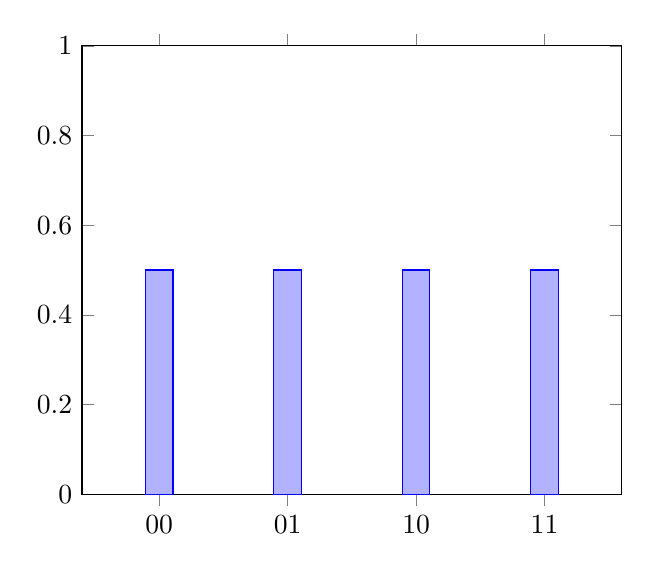
\begin{tikzpicture}
        \begin{axis}[
                ybar,
                ymax=1,
                ymin=0,
                symbolic x coords = {00,01,10,11},
                enlarge x limits=0.2
        ]
        \addplot+ coordinates {(00, 0.5) (01, 0.5) (10, 0.5) (11, 0.5)};
        \end{axis}
        \end{tikzpicture}
        }

        $\frac{1}{2} \Big (\ket{00} + \ket{01} + \alert{\ket{10}} + \ket{11} \Big )$
        \end{center}
\end{frame}

\begin{frame}{Key Ideas: Interference pt. I}
        \begin{center}
                Inversion about the \alert{\underline{mean}}: ($x \mapsto (-x +  mean) + mean$)

                \vspace{0.4cm}
                \hspace{-1cm}
        \scalebox{0.7}{
        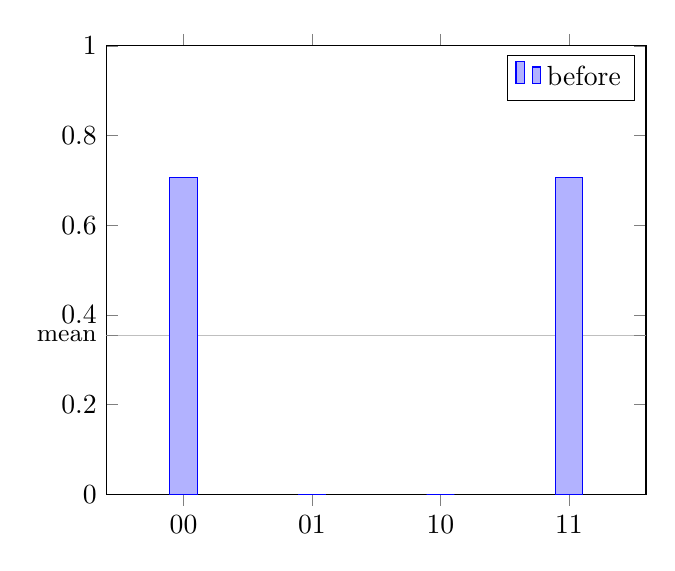
\begin{tikzpicture}
        \begin{axis}[
                ybar,
                ymax=1,
                ymin=0,
                symbolic x coords = {00,01,10,11},
                enlarge x limits=0.2,
                extra y ticks       = 0.3535,
                extra y tick labels = \small{mean},
                extra y tick style  = { grid = major }
        ]
        \addplot+ coordinates {(00, 0.707) (01, 0) (10, 0) (11, 0.707)};  
        \legend{before}
        \end{axis}
        \end{tikzpicture}
        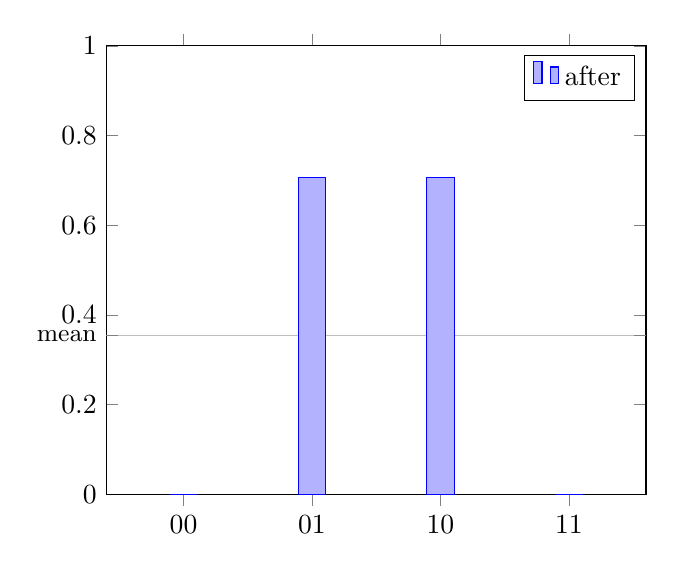
\begin{tikzpicture}
        \begin{axis}[
                ybar,
                ymax=1,
                ymin=0,
                symbolic x coords = {00,01,10,11},
                enlarge x limits=0.2,
                extra y ticks       = 0.3535,
                extra y tick labels = \small{mean},
                extra y tick style  = { grid = major }
        ]
        \addplot+ coordinates {(00, 0) (01, 0.7070) (10, 0.7070) (11, 0)};  
        \legend{after}
        \end{axis}
        \end{tikzpicture}
        }

        Intuitively mass of some states was given to others
        \end{center}
\end{frame}

\begin{frame}{Key Ideas: Interference pt. II}
        \begin{center}
              Mind the following particular case of inversion about the mean 

                \vspace{0.4cm}
                \hspace{-1cm}
        \scalebox{0.7}{
        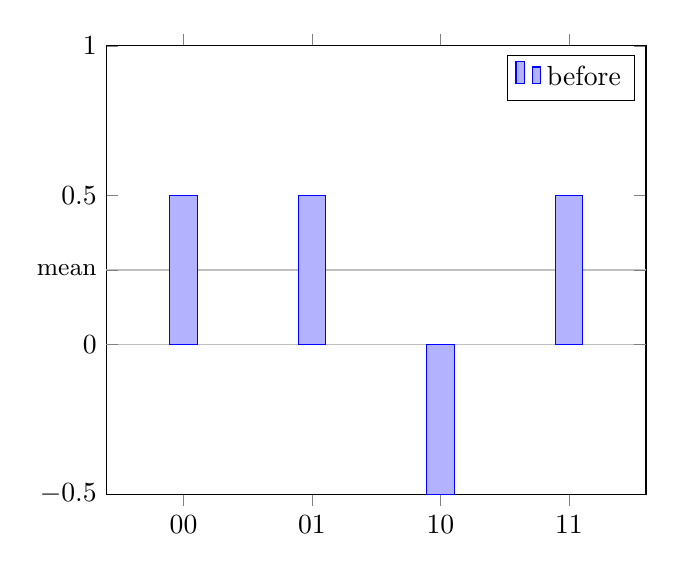
\begin{tikzpicture}
        \begin{axis}[
                ybar,
                ymax=1,
                ymin=-0.5,
                symbolic x coords = {00,01,10,11},
                enlarge x limits=0.2,
                extra y ticks       = {0.25,0},
                extra y tick labels = {\small{mean},{}},
                extra y tick style  = { grid = major }
        ]
        \addplot+ coordinates {(00, 0.5) (01, 0.5) (10, -0.5) (11, 0.5)};  
        \legend{before}
        \end{axis}
        \end{tikzpicture}
        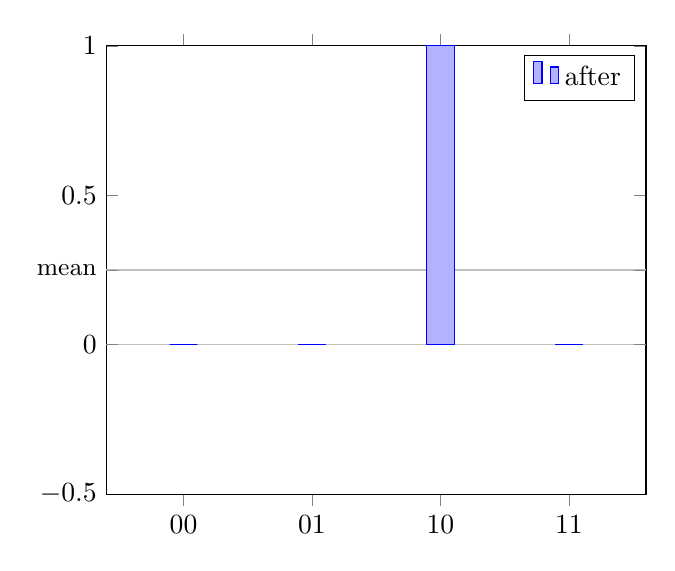
\begin{tikzpicture}
        \begin{axis}[
                ybar,
                ymax=1,
                ymin=-0.5,
                symbolic x coords = {00,01,10,11},
                enlarge x limits=0.2,
                extra y ticks       = {0.25,0},
                extra y tick labels = {\small{mean},{}},
                extra y tick style  = { grid = major }
        ]
        \addplot+ coordinates {(00, 0.0) (01, -0.0) (10, 1) (11, 0.0)};  
        \legend{after}
        \end{axis}
        \end{tikzpicture}
        }
        
        Intuitively, mass of wrong answers was given to the right one 
        \end{center}

\end{frame}

\section{Putting inversion into practice}

\begin{frame}{The Steps}
        \begin{enumerate}
                \item Put all possible answers in uniform superposition
                \item Negate \alert{phases} of the \alert{right answer}
                \item Invert about the mean
                \item \alert{Repeat} steps $2$ and $3$ until ensured we will
                        measure the right answer with high probability
                        ($\approx \sqrt{2^n}$ times)
        \end{enumerate}
\end{frame}

\begin{frame}{The Circuit}

        \begin{center}
                \hspace{0.2cm}
                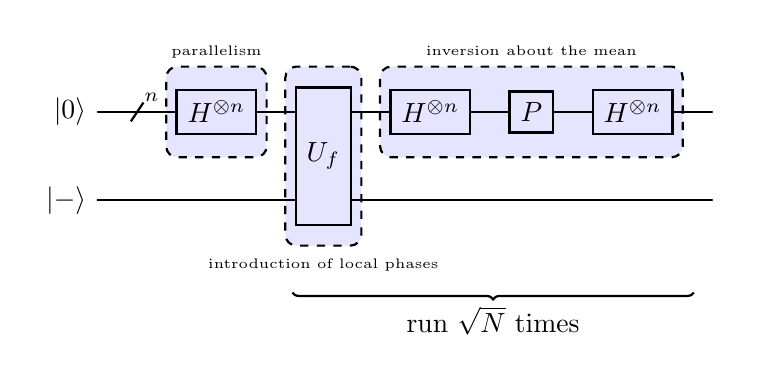
\begin{tikzpicture}
                  \node{
                        \begin{quantikz}[transparent]
                                \lstick{\ket{0}} &[5mm] \gate{H^{\otimes n}} \qwbundle{n} 
                                \gategroup[wires=1,steps=1,style={dashed,
                                rounded corners,fill=blue!10, inner xsep=0.2pt},background]
                                {\tiny{parallelism}}
                                & \gate[wires=2]{U_f} \gategroup[wires=2,steps=1,style={dashed,
                                rounded corners,fill=blue!10, inner xsep=0.2pt}, 
                                label style={label position = 
                                below, yshift=-0.4cm},background]
                                {\tiny{introduction of local phases}}
                                & \gate{H^{\otimes n}} 
                                \gategroup[wires=1,steps=3,style={dashed,
                                rounded corners,fill=blue!10, inner xsep=0.2pt},background]{
                                \tiny{inversion about the mean}}
                                & \gate{P} & \gate{H^{\otimes n}} & \qw  \\
                                \tikzmark{x1} \lstick{$\ket{-}$} \tikzmark{x2}
                                & \qw & & \qw & \qw & \qw & \qw 
                        \end{quantikz}
                };
                    \draw [
                    thick,
                    decoration={
                        brace,
                        mirror,
                        raise=0.5cm
                    },
                    decorate
                    ] (-1.1,-1.2) -- (4,-1.2) 
                    node [pos=0.5,anchor=north,yshift=-0.55cm] {run $\sqrt{N}$ times};
              \end{tikzpicture}
        \end{center} 

        \begin{tikzpicture}[overlay,remember picture,
        box/.style = {rounded corners},
        pin edge={-Stealth,thick, red}]
        \coordinate (x1) at ($({pic cs:x1})+(+0.0ex, 1.5ex)$);
        \coordinate (x2) at ($({pic cs:x2})+(-5.5ex,-1.5ex)$);
        \node[semitransparent, 
             fit=(x1) (x2),
             pin=below:\tiny{Eigenvector of $U_f$ with $-1$ as eigenvalue}]  {};
       \end{tikzpicture}

       {\scriptsize
       \textbf{N.B.} It is often convenient to omit the bottom qubit}

\end{frame}

\begin{frame}{Adding Local Phases}

        Recall from last lectures the notion of phase
        kickback and that
        \[
                U_f \ket{x} \ket{-} = (-1)^{f(x)} \ket{x} \ket{-}
        \]
        
        In particular, if $x$ is as \alert{solution} of $f$ we obtain a \alert{phase flip}
        \[
                U_f \ket{x} \ket{-} = (-1) \ket{x} \ket{-}
        \]

\end{frame}

\begin{frame}{Inversion About the Mean pt. I}
        We start with the operation that phase flips
        basis states different from $\ket{0}$, \ie\
        \[
                P = 2 \ket{0}\bra{0} - I
        \]
        Then we calculate
        \begin{flalign*}
             &\,   H^{\otimes n} (2 \ket{0} \bra{0} - I) H^{\otimes n} & \\
             & = (H^{\otimes n} (2 \ket{0} \bra{0}) - H^{\otimes n}) H^{\otimes n} & \\
             & = H^{\otimes n} (2 \ket{0} \bra{0}) H^{\otimes n} - H^{\otimes n} H^{\otimes n} & \\
             & = 2 H^{\otimes n} \ket{0} \bra{0} H^{\otimes n} - I
        \end{flalign*}
        Denoting $H^{\otimes n} \ket{0}$ by $\ket{\psi}$ we obtain,
        \[
                2 \ket{\psi} \bra{\psi} - I
        \]
\end{frame}

\begin{frame}{Inversion About the Mean pt. II}

        \begin{enumerate}

                \item Prove that $\ket{\psi}\bra{\psi} = \frac{1}{N} \sum_{x,y
                        \in N} \ket{x}\bra{y}$ with $N = 2^n$

                \item Prove that $2\ket{\psi}\bra{\psi} -
                          I$ is the desired inversion about the mean
\end{enumerate}
\end{frame}

\begin{frame}{Inversion About the Mean pt. III}

        \begin{flalign*}
                & \,\textstyle{ \Big (2 \frac{1}{N} \sum_{x,y \in N} \ket{x} \bra{y} - I \Big ) 
                \sum_{k \in N} \alpha_k \ket{k} } & \\
                & = \textstyle { 2 \frac{1}{N} \sum_{x,y \in N} \ket{x}\bra{y} 
                \Big ( \sum_{k \in N} \alpha_k \ket{k} \Big ) - \sum_k \alpha_k \ket{k} } &  \\
                & = \textstyle { 2 \frac{1}{N} \sum_{x,y \in N} 
                \Big ( \sum_{k \in N} \alpha_k \langle y,k \rangle \ket{x} \Big ) - 
                \sum_k \alpha_k \ket{k} } & \\
                & = \textstyle { 2 \frac{1}{N} \sum_{x,y \in N} 
                \alpha_y \ket{x} - 
                \sum_k \alpha_k \ket{k} } & \\
                & = \textstyle { 
                        2 \underbrace{\frac{1}{N} \sum_{y \in N} \alpha_y}_{\text{\alert{mean} - } \alpha} 
                        \sum_{x \in N}  \ket{x} - \sum_k \alpha_k \ket{k} } & \\
                & = \textstyle { 
                \sum_{x \in N} 2 \alert{\alpha}  \ket{x} - \sum_k \alpha_k \ket{k} } &  \\
                & = \textstyle { 
        \sum_{k \in N} (- \alpha_k + 2 \alert{\alpha}) \ket{k} } &  
        \end{flalign*}
\end{frame}

\begin{frame}{Example: $N = 2^3 = 8, w = 011$}
        \scalebox{0.7}{
                \hspace{-0.5cm}
        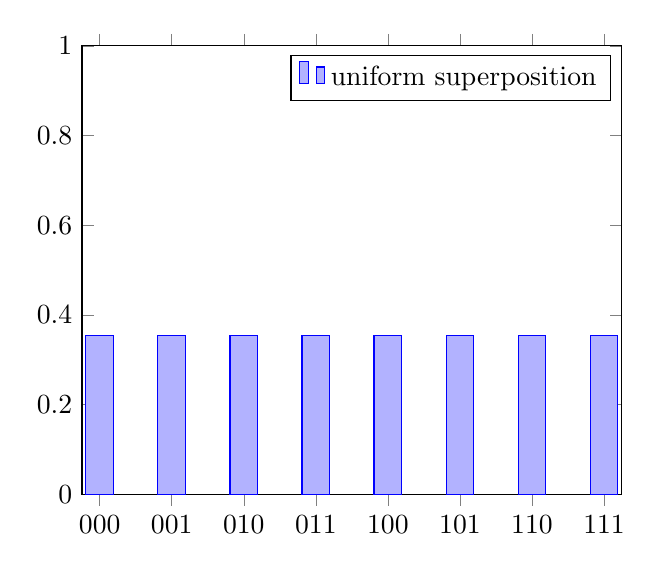
\begin{tikzpicture}
        \begin{axis}[
                ybar,
                ymax=1,
                ymin=0,
                symbolic x coords = {000,001,010,011,100,101,110,111},
                enlarge x limits=0.035
        ]
        \addplot+ coordinates {(000, 0.3535) (001, 0.3535) (010, 0.3535) (011, 0.3535)
                (100,0.3535) (101,0.3535) (110,0.3535) (111,0.3535)};  
        \legend{uniform superposition}
        \end{axis}
        \end{tikzpicture}
        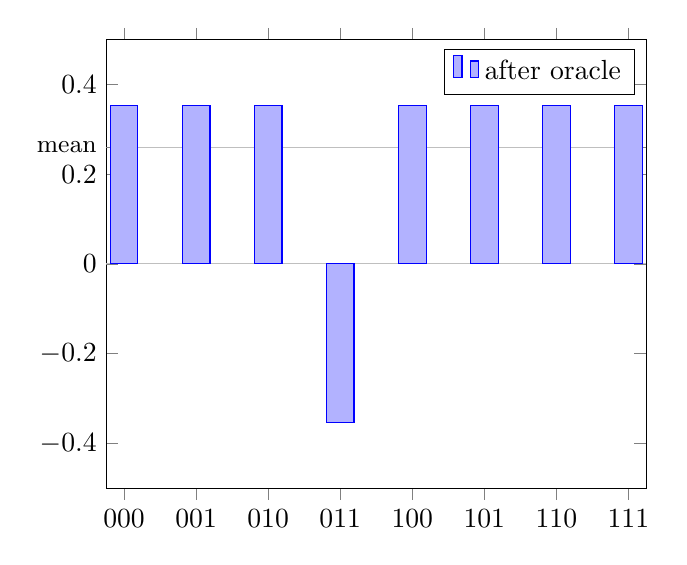
\begin{tikzpicture}
        \begin{axis}[
                ybar,
                ymax=0.5,
                ymin=-0.5,
                extra y ticks       = {0.26,0},
                extra y tick labels = {\small{mean},{}},
                extra y tick style  = { grid = major },
                symbolic x coords = {000,001,010,011,100,101,110,111},
                enlarge x limits=0.035
        ]
        \addplot+ coordinates {(000, 0.3535) (001, 0.3535) (010, 0.3535) (011, -0.3535)
                (100,0.3535) (101,0.3535) (110,0.3535) (111,0.3535)};  
        \legend{after oracle}
        \end{axis}
        \end{tikzpicture}

}
 
\end{frame}

\begin{frame}{Example: $N = 2^3 = 8, w = 011$}
        \scalebox{0.7}{
                \hspace{-0.6cm}
        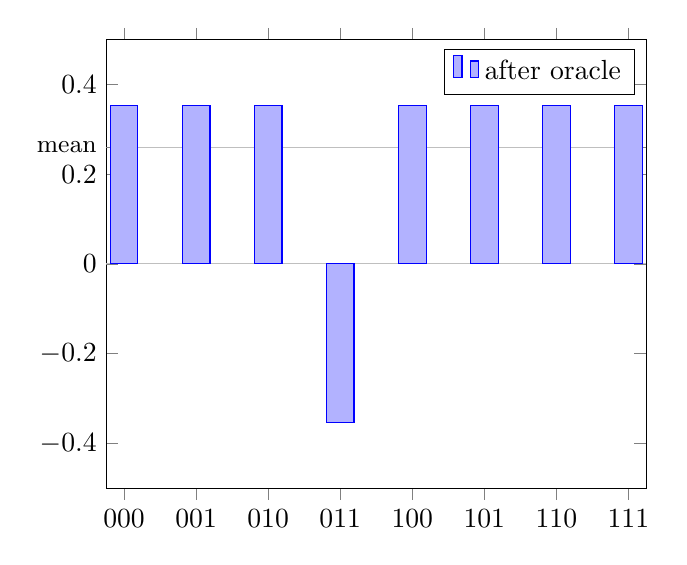
\begin{tikzpicture}
        \begin{axis}[
                ybar,
                ymax=0.5,
                ymin=-0.5,
                extra y ticks       = {0.26,0},
                extra y tick labels = {\small{mean},{}},
                extra y tick style  = { grid = major },
                symbolic x coords = {000,001,010,011,100,101,110,111},
                enlarge x limits=0.035
        ]
        \addplot+ coordinates {(000, 0.3535) (001, 0.3535) (010, 0.3535) (011, -0.3535)
                (100,0.3535) (101,0.3535) (110,0.3535) (111,0.3535)};  
        \legend{after oracle}
        \end{axis}
        \end{tikzpicture}
        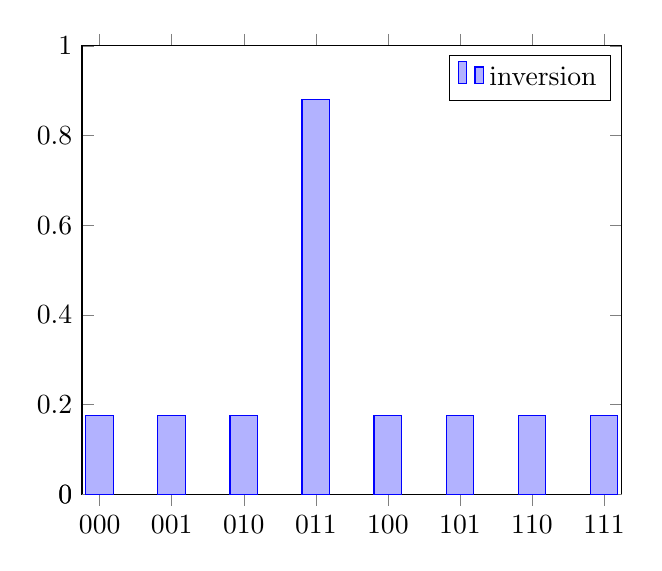
\begin{tikzpicture}
        \begin{axis}[
                ybar,
                ymax=1,
                ymin=0,
                extra y ticks       = {0},
                symbolic x coords = {000,001,010,011,100,101,110,111},
                enlarge x limits=0.035
        ]
        \addplot+ coordinates {(000, 0.176) (001, 0.176) (010, 0.176) (011, 0.88)
                (100,0.176) (101,0.176) (110,0.176) (111,0.176)};  
        \legend{inversion}
        \end{axis}
        \end{tikzpicture}

}
 
\end{frame}

\begin{frame}{Example: $N = 2^3 = 8, w = 011$}
        \scalebox{0.7}{
                \hspace{-0.7cm}
       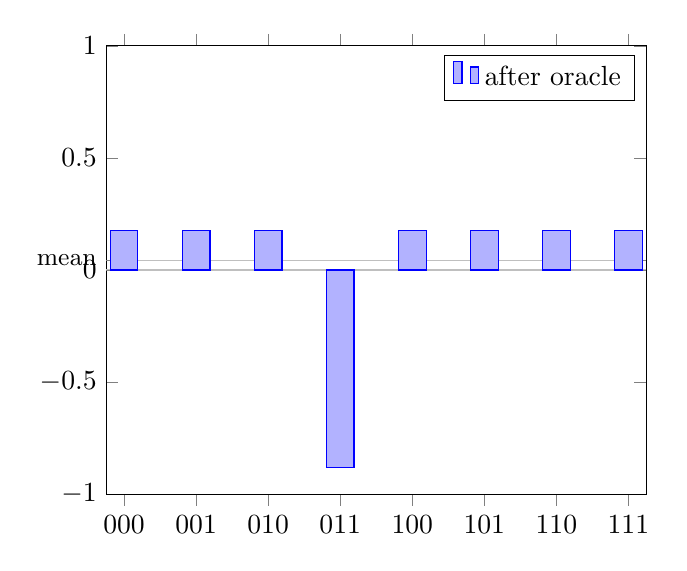
\begin{tikzpicture}
        \begin{axis}[
                ybar,
                ymax=1,
                ymin=-1,
                extra y ticks       = {0.044,0},
                extra y tick labels = {\small{mean},{}},
                extra y tick style  = { grid = major },
                symbolic x coords = {000,001,010,011,100,101,110,111},
                enlarge x limits=0.035
        ]
        \addplot+ coordinates {(000, 0.176) (001, 0.176) (010, 0.176) (011, -0.88)
                (100,0.176) (101,0.176) (110,0.176) (111,0.176)};  
        \legend{after oracle}
        \end{axis}
        \end{tikzpicture}
        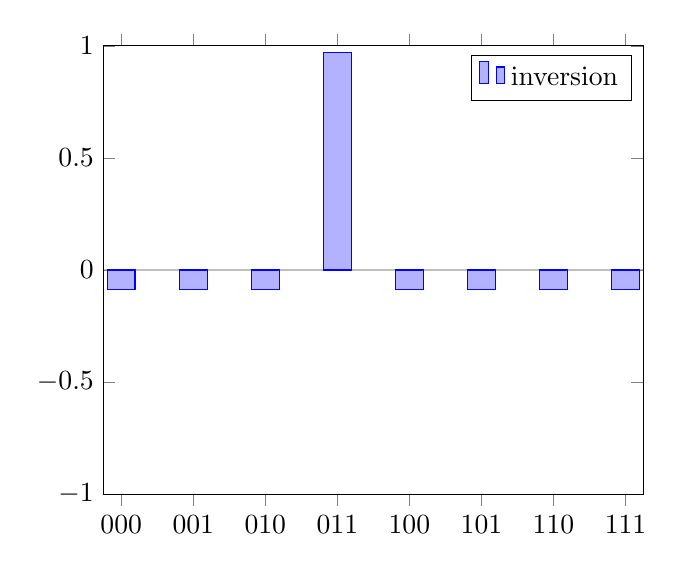
\begin{tikzpicture}
        \begin{axis}[
                ybar,
                ymax=1,
                ymin=-1,
                extra y ticks       = {0},
                extra y tick labels = {{}},
                extra y tick style  = { grid = major },
                symbolic x coords = {000,001,010,011,100,101,110,111},
                enlarge x limits=0.035
        ]
        \addplot+ coordinates {(000, -0.088) (001, -0.088) (010, -0.088) (011, 0.972)
                (100,-0.088) (101,-0.088) (110,-0.088) (111,-0.088)};  
        \legend{inversion}
        \end{axis}
        \end{tikzpicture}

}
 
        \vspace{0.5cm}
        At the end probability of measuring $011$ is $\approx 94.5\%$
\end{frame}

\section{Grover's performance}

\begin{frame}{Setting the Stage pt. I}

        In order to further analyse Grover's algorithm, it is useful to take a
        \alert{$2$-dimensional geometrical} perspective
        
        \pause
        Take the vectors \alert{$\ket{w}$} and $\alert{\ket{r}} =
        \frac{1}{\sqrt{N-1}} \sum_{x \not = w} \ket{x}$. We obtain a
        $2$-dimensional vector space with orthonormal basis
        $\{\ket{w},\ket{r}\}$

        \pause
        Additionally, the uniform superposition $\ket{\psi}$ can be rewritten
        as
        \[
                \textstyle{
                \frac{1}{\sqrt{N}} \ket{w} + \sqrt{\frac{N-1}{N}} \ket{r}
        }
        \]

        \pause
        This gives \dots
\end{frame}

\begin{frame}{Setting the Stage pt. II}

        \begin{center}
        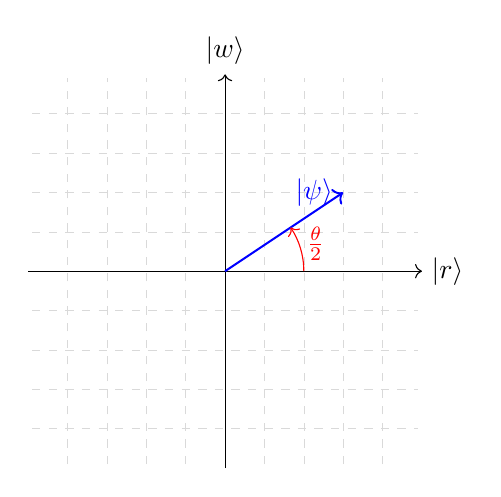
\begin{tikzpicture}[scale=0.5]
            \draw[help lines, color=gray!30, dashed] (-4.9,-4.9) grid (4.9,4.9);
            \draw[->] (-5,0)--(5,0) node[right]{$\ket{r}$};
            \draw[->] (0,-5)--(0,5) node[above]{$\ket{w}$};
            \draw[name path=fr, blue,->,line width = 0.25mm] (0,0) -- (3,2) 
                    node[left]{$\ket{\psi}$};
            \path[name path=circ] (0,0) circle (2);
            \draw[red, ->, intersection segments={of=circ and fr, sequence=L1}];
            \node[red] at (2.3,0.7) {$\frac{\theta}{2}$};
        \end{tikzpicture}
        \end{center}

        where $\sin(\frac{\theta}{2}) = \frac{1}{\sqrt{N}}$. Our goal is to rotate
        the vector to become \alert{as close as possible} to $\ket{w}$
\end{frame}

\end{document}
